\authoredsubsection{Sprint 1}{Julius}{Julius Bethge}\label{sec:sprint1}

\subsubsection{Sprint Goal and Planning}\label{sec:sprint1-goal}

Sprint 1 ran from 28 April to 11 May 2026, with Julius acting as Scrum Master. Following the preliminary organization in Sprint 0, it focused on setting up the working environment, conducting the initial research, forming a first view of the pipeline architecture, and taking the first steps toward the showcase interface. The sprint goal combined five workstreams: establishing the project and development environment, delivering a first showcase-application increment, clarifying access to suitable language models, defining relevant evaluation metrics, and deriving an initial pipeline architecture from scientific research. The sprint was initially planned with 25 story points, corresponding to five points for each team member. Its purpose was to reduce the principal uncertainties of the project rather than to deliver a complete pipeline.

Responsibilities followed the main components: Marco established Jira and researched judges and their biases; Julius created the repositories and initial application and coordinated the sprint; Mohsin investigated model providers; Sebastian covered local models and routing; and Gáspár developed the metrics and optimizer research. The architecture, MVP, repository strategy, and Sprint Review were collaborative.

\Cref{fig:sprint1-backlog} shows the six work items recorded in Jira at the end of the sprint, including the additional two-point task for establishing a local LLM setup after no external token provider was available.

\begin{figure}
\centering
\pandocbounded{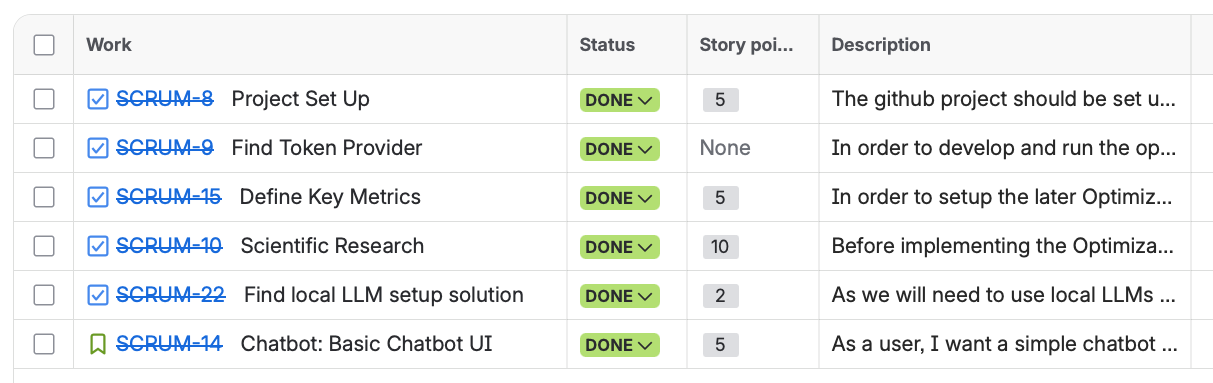
\includegraphics[keepaspectratio]{assets/sprints/sprint1-backlog.png}}
\caption{Sprint 1 backlog in Jira showing story-point estimates and completion status.}
\label{fig:sprint1-backlog}
\end{figure}

\subsubsection{Implementation and Sprint Execution}\label{sec:sprint1-execution}

The team created the \texttt{LMUxInterhyp} GitHub organization with two repositories serving different purposes. The \texttt{pipeline} repository provided an experimental environment for rapidly exploring Router, judge, and optimization approaches. The \texttt{chatbot} repository formed the maintainable codebase for the integrated showcase application. Validated ideas could therefore be reimplemented in the application without treating exploratory Python code as its foundation. Jira issues were linked to branches and pull requests, supported by automated checks and preview deployments.

The first application increment combined a React and TypeScript frontend with a Convex backend. It already allowed a user to submit a query and receive an LLM-generated answer. Ollama supported local execution, while OpenRouter was available for the first deployed setup. The increment established the technical basis for the showcase application, but it did not yet contain the multi-stage Router, judge, or optimizer.

Model access was a critical dependency because the Router, agents, judge, and optimizer could each require inference. Neither Interhyp nor the university could provide the required tokens. The team therefore selected Ollama as the initial local runtime and documented suitable models and setup instructions. This removed the immediate dependency on an external API budget. It was not intended as a permanent architectural restriction because the planned components could require different model capabilities.

The metric work translated the objective into routing quality, latency, and cost. Candidate measures included routing accuracy, agent-level precision and recall, clarification behavior, Router latency, and token cost. Broader measures included first-touch resolution and cost per successful outcome. Because Interhyp reported uneven agent usage, aggregate accuracy could conceal weak performance on less frequent agents. Weighted and agent-level results were therefore retained for later evaluation, while no combined optimization metric was fixed during this sprint.

Research covered multi-agent routing, LLM-based evaluation, judge bias, prompt optimization, and self-improving pipelines. The team used these workstreams to compare possible approaches and translate them into requirements for the initial architecture. The resulting proposal treated routing as a decision involving quality, latency, and cost, considered an independent judge as a source of evaluation signals, and investigated automated prompt optimization as an alternative to repeated manual refinement. Judge panels and more advanced learning approaches were retained as possible extensions rather than included in the initial MVP.

The initial production-path concept used a Router to select the specialist agent best suited to a user query. The selected agent would generate the response returned to the user, while alternative agents remained available for other request types.

\begin{figure}
\centering
\pandocbounded{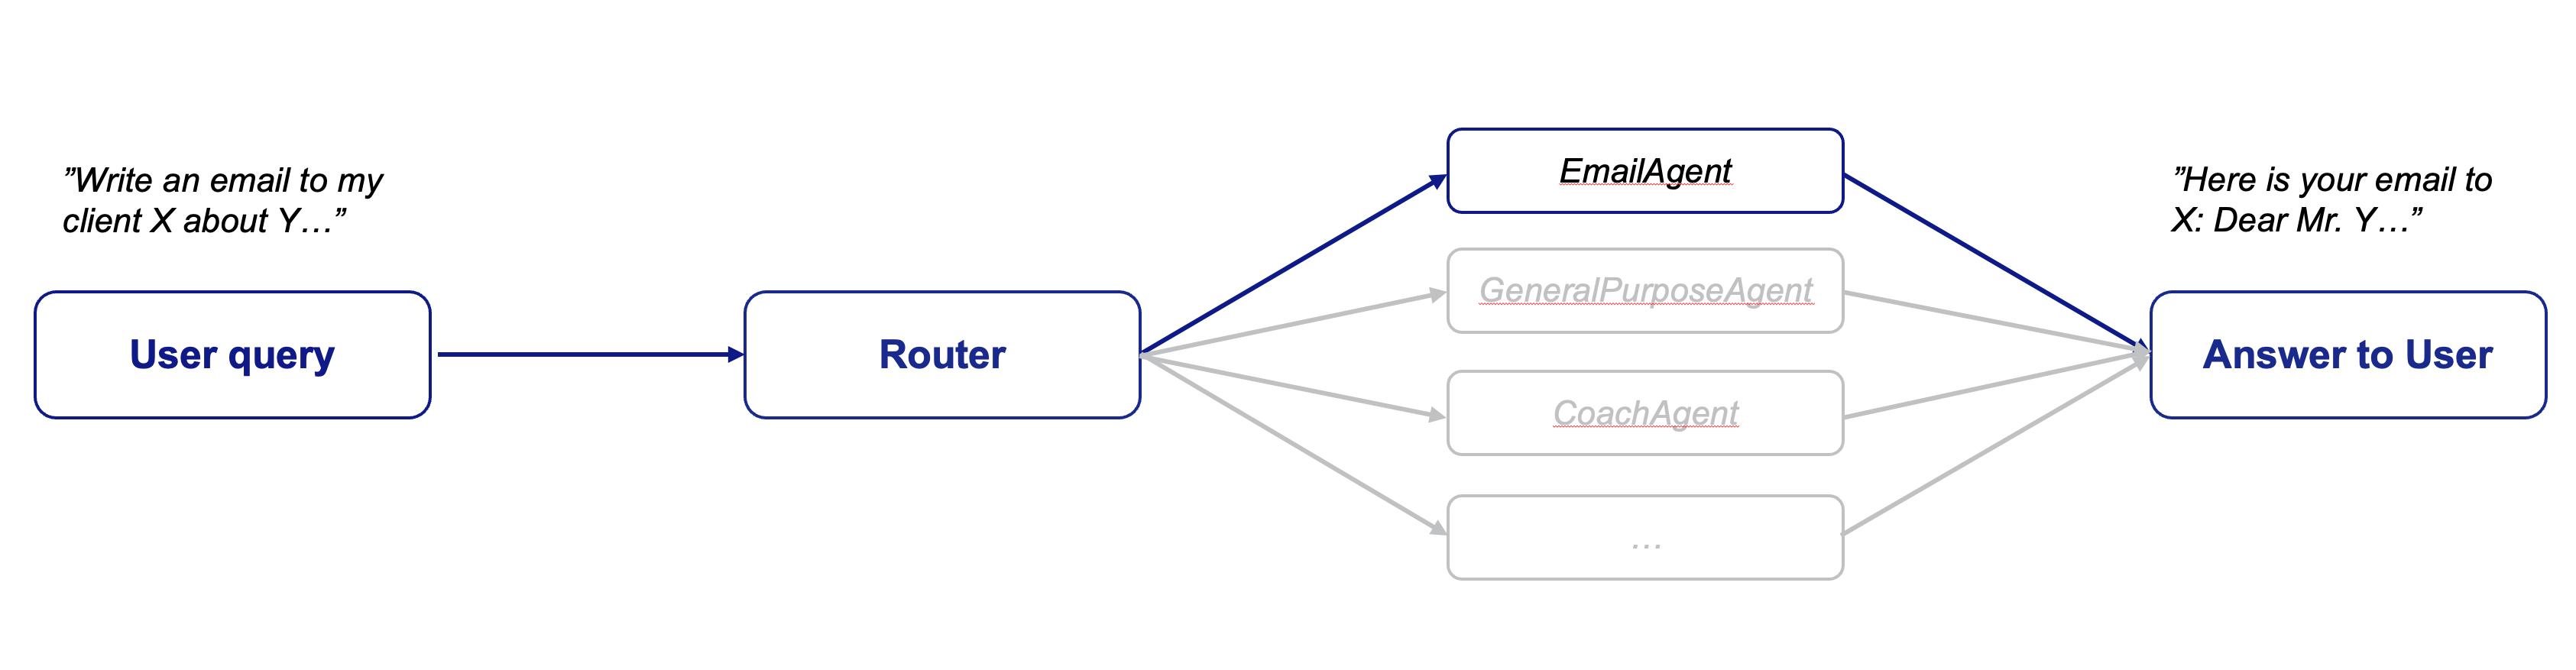
\includegraphics[keepaspectratio]{assets/sprints/sprint1-production-path.png}}
\caption{Initial Sprint 1 production path from a user query to the selected specialist agent's response.}
\label{fig:sprint1-production-path}
\end{figure}

The broader proposal extended this production path with a separate asynchronous pipeline. The live path would route a query and return an agent answer without waiting for evaluation. It would also create a structured trace containing the query, routing decision, candidate information, and answer. The asynchronous path could compare alternative outcomes, derive evaluation signals through an independent judge, and optimize the Router prompt. Resulting changes would require validation before deployment.

\subsubsection{Sprint Review}\label{sec:sprint1-review}

The Sprint Review took place on 12 May 2026 with our Interhyp partners. During the sprint, the lack of provided inference tokens had made an additional local-model setup task necessary. This increased the scope from 25 to 27 story points. All 27 points were completed. The team presented the project and repository setup, first chatbot increment, metric proposal, scientific findings, initial architecture, and MVP boundary.

\Cref{fig:sprint1-burndown} shows the scope increase and the completion of all committed work by the end of the sprint.

\begin{figure}
\centering
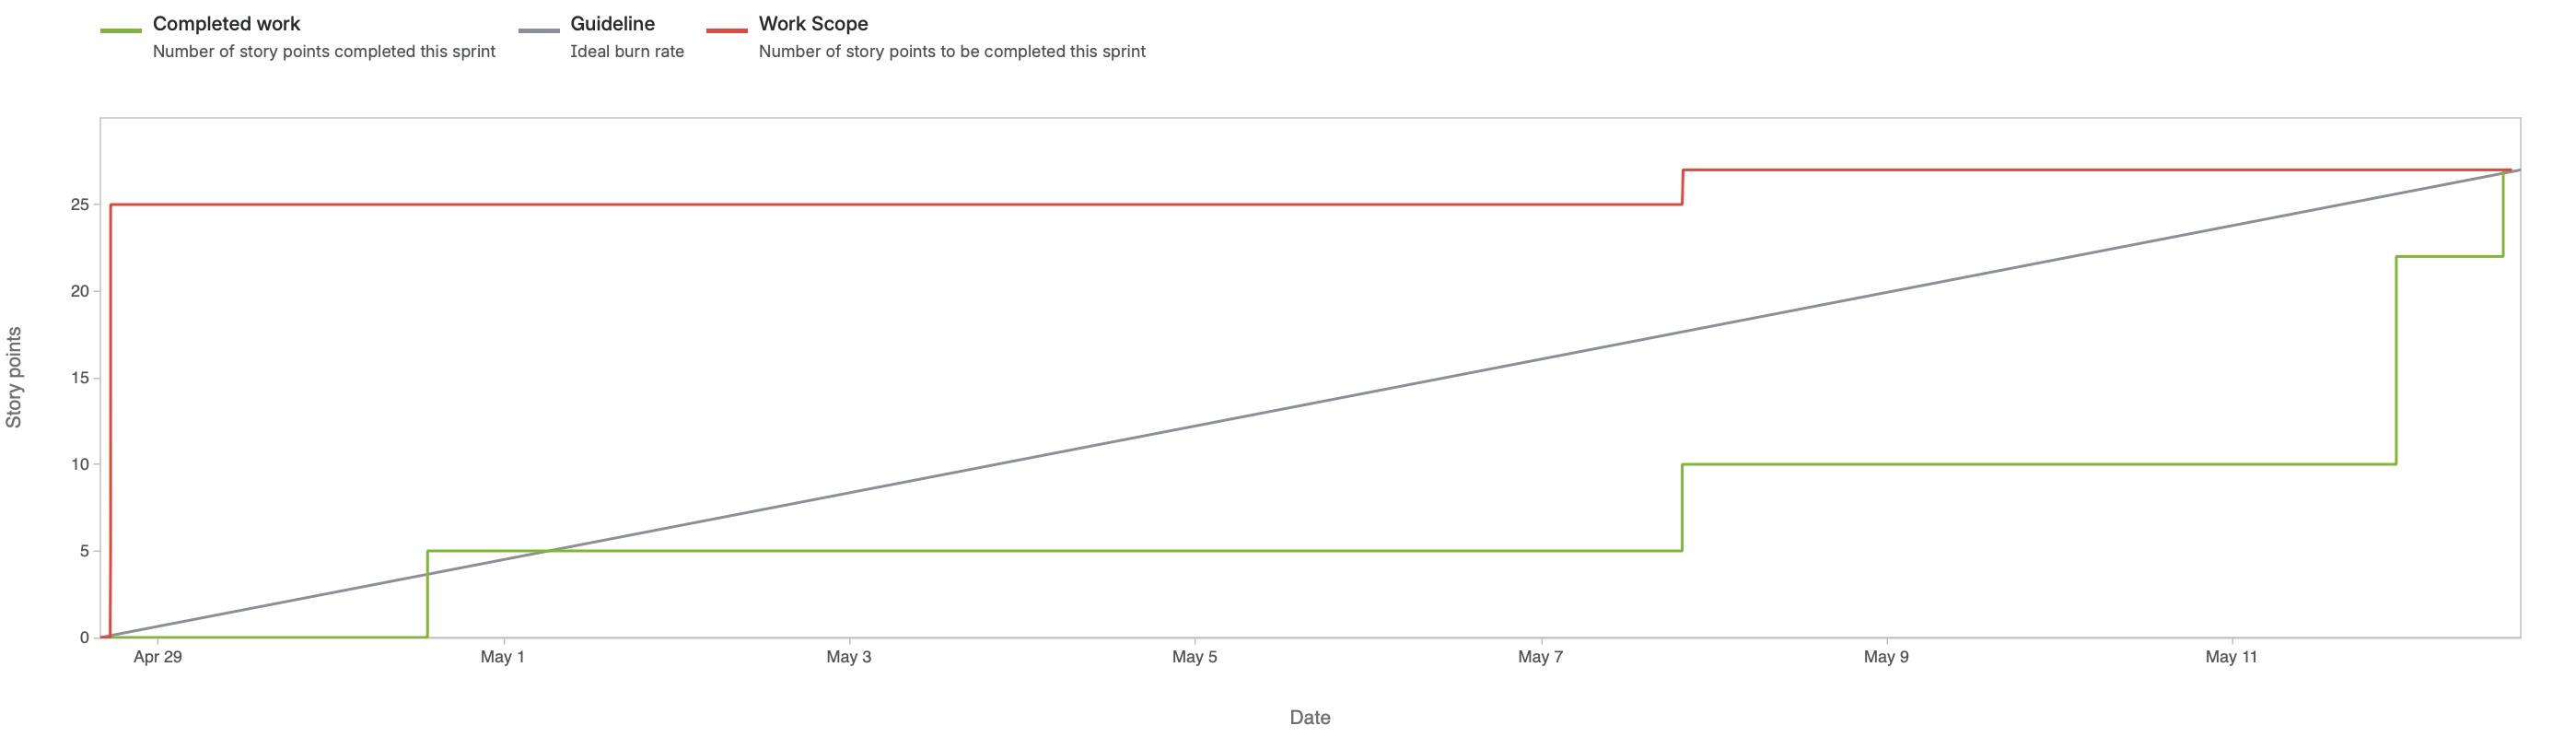
\includegraphics[width=1\linewidth,height=\textheight,keepaspectratio]{assets/sprints/sprint1-burndown.png}
\caption{Sprint 1 burnup chart.}\label{fig:sprint1-burndown}
\end{figure}

The discussion concentrated on the architecture rather than on the basic chatbot interface. Interhyp considered the separation between the live application path and asynchronous evaluation and optimization a suitable basis for the following sprints. They also supported the MVP approach, which prioritized a smaller executable pipeline before more advanced routing and judge concepts. At the same time, the architecture remained open to revision as the components were implemented and evaluated.

The review also reinforced the need to interpret accuracy in the context of unequal agent usage. This supported the planned use of agent-level and potentially weighted evaluation alongside aggregate results. Overall, the positive review allowed Sprint 2 to move from setup and architectural reasoning toward the first implementation of the pipeline components, data, Router, judge, and optimizer.

\subsubsection{Sprint Retrospective}\label{sec:sprint1-retrospective}

The retrospective showed high motivation, broad participation, and productive collaboration. Team members particularly valued the brainstorming process, the effective division of work, and the contributions to the research and architecture. These strengths had enabled the team to address several foundational questions within one sprint and to present a coherent direction despite the unresolved model-access issue at its beginning.

The team nevertheless identified a need for clearer task delegation, better-prepared meeting agendas, and more opportunities for in-person work. It also concluded that meetings with Interhyp should make more active use of the partners' expertise. Rather than primarily presenting progress, the team wanted to prepare concrete questions and alternatives that could be discussed with them. The complete feedback board is shown in \cref{fig:sprint1-retrospective-feedback}.

\begin{center}
\centering
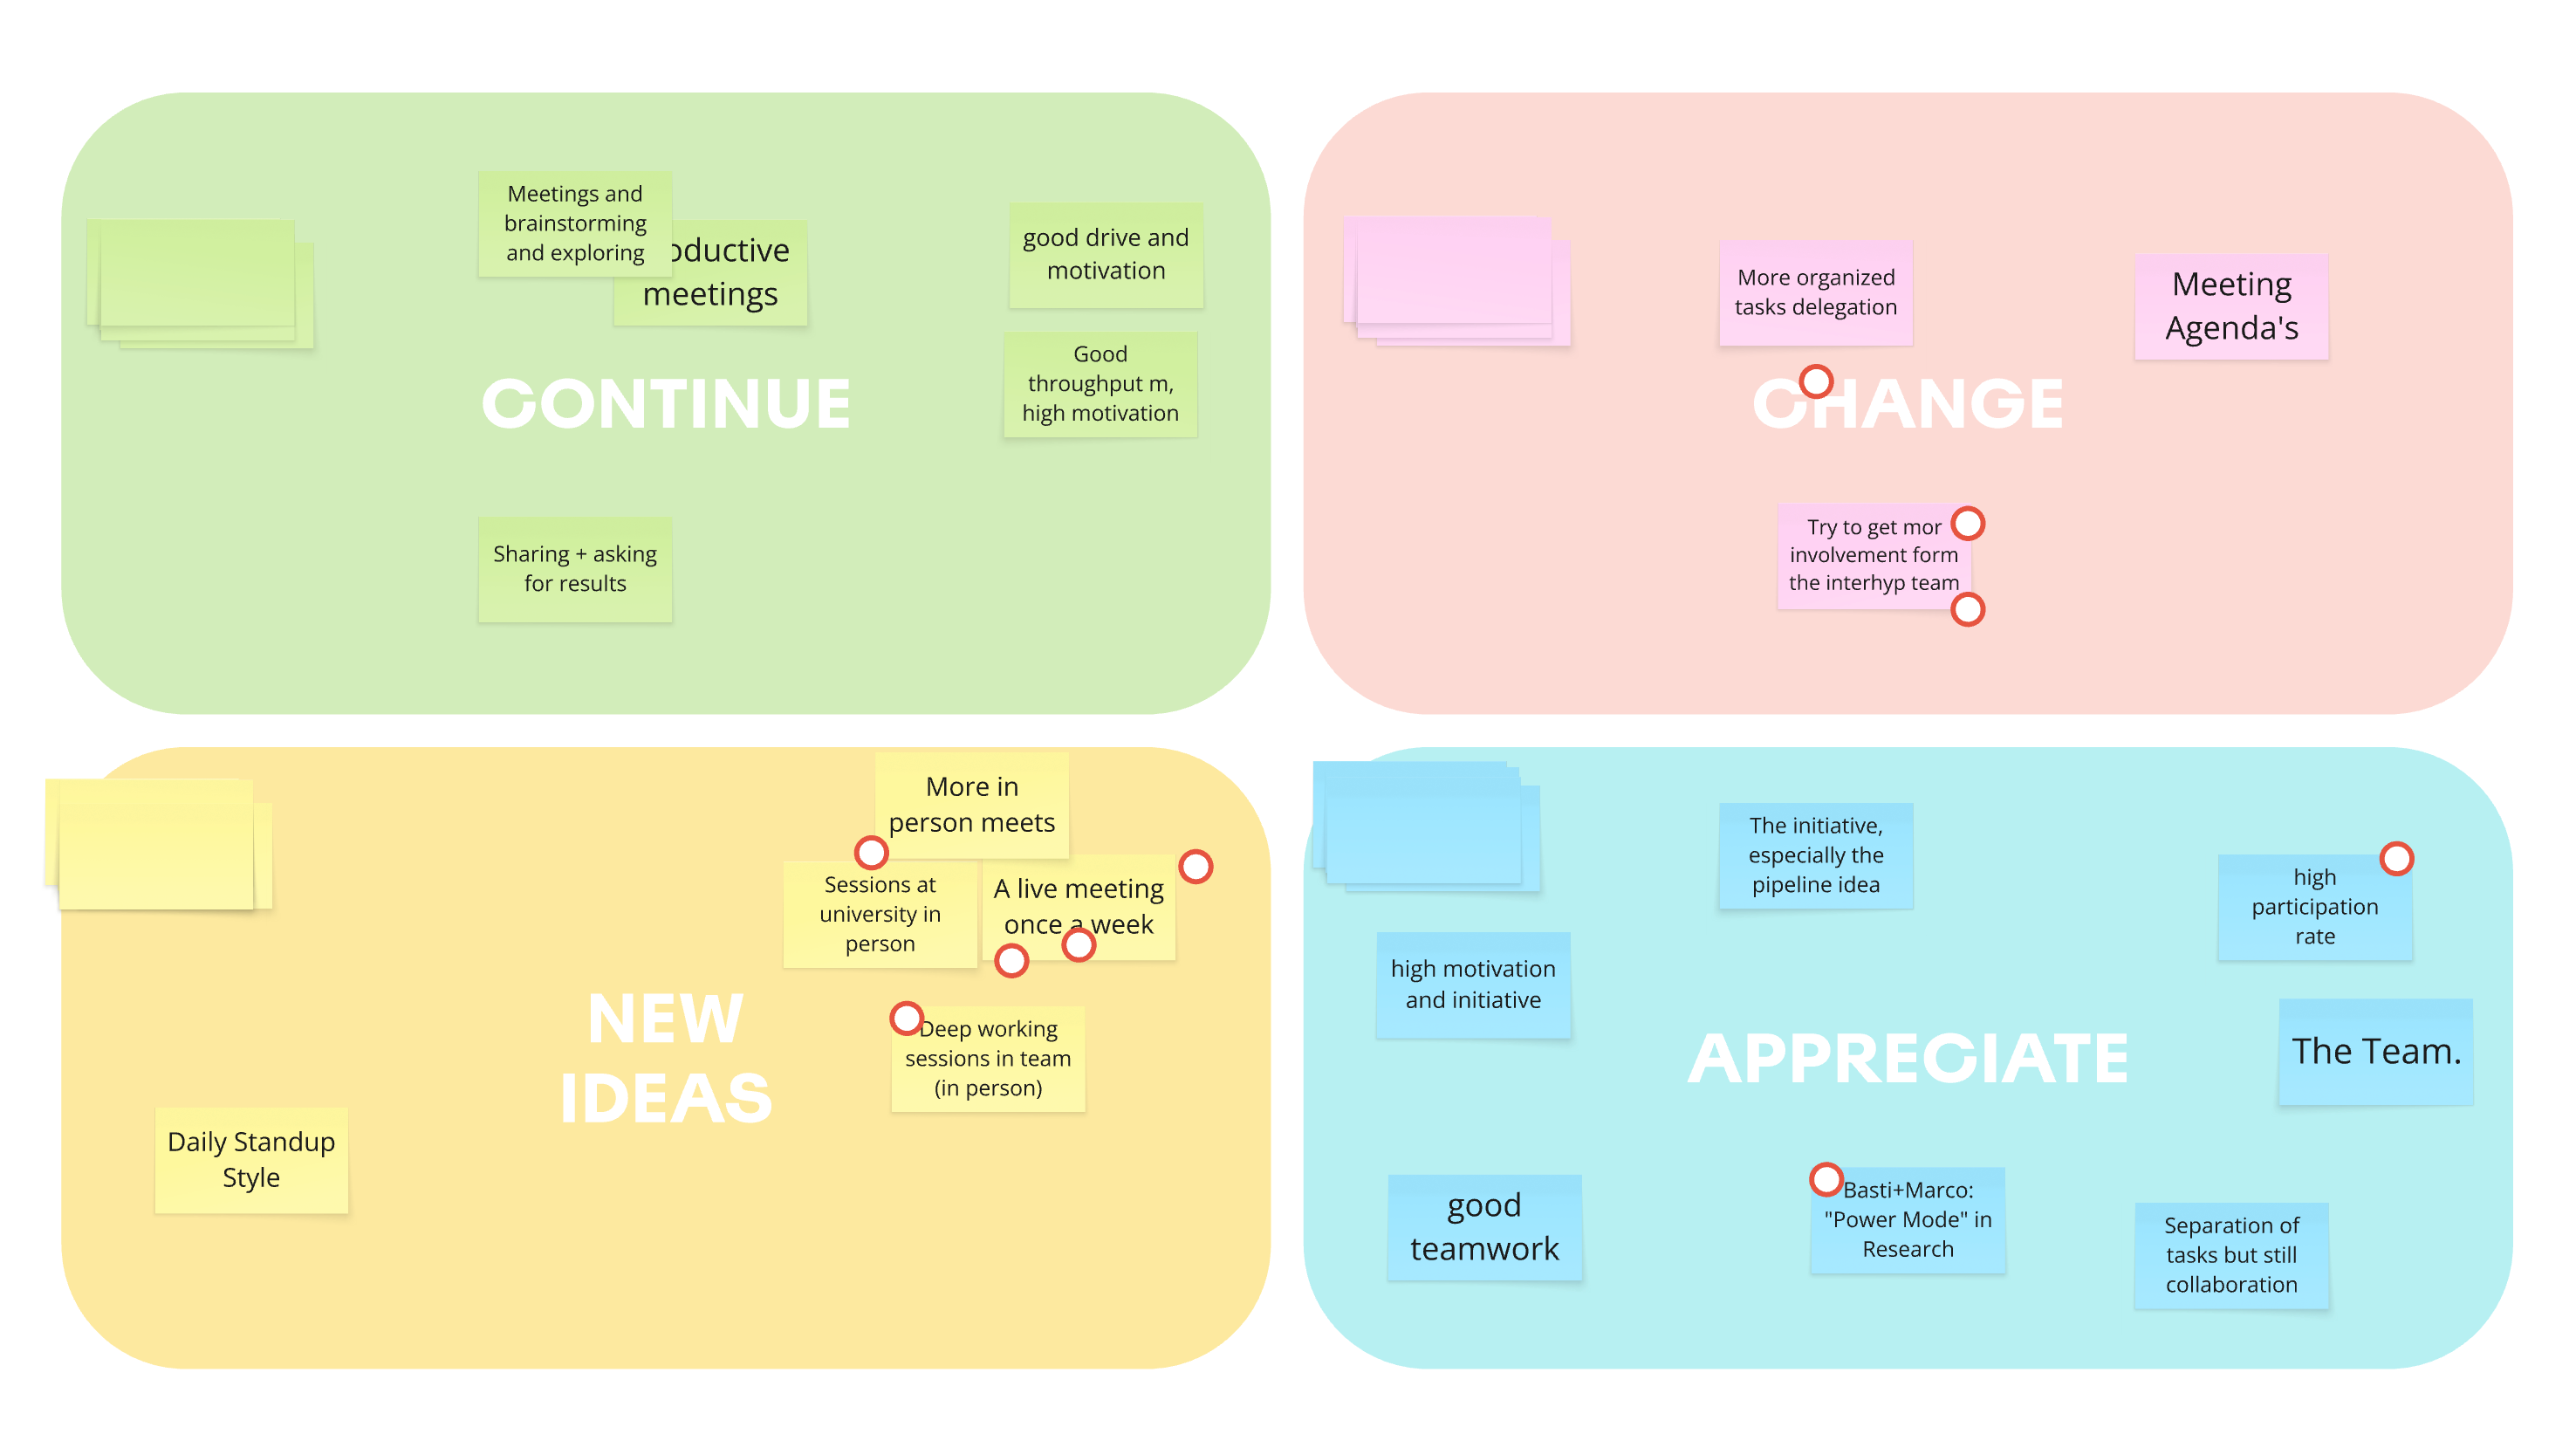
\includegraphics[width=1\linewidth,height=\textheight,keepaspectratio]{assets/sprints/sprint1-retrospective-feedback.png}
\captionof{figure}{Sprint 1 retrospective board showing feedback grouped as Continue, Change, New Ideas, and Appreciate.}
\label{fig:sprint1-retrospective-feedback}
\end{center}

Two actions were adopted for Sprint 2. First, a recurring in-person working session on Tuesdays would provide time for deeper collaboration and architectural alignment. Second, Interhyp meetings would be prepared as focused discussion and feedback sessions. These changes were intended to improve shared understanding within the team, shorten coordination paths, and incorporate domain feedback earlier into technical decisions. \Cref{fig:sprint1-retrospective-actions} records the owners and deadlines agreed for both actions.

\begin{center}
\centering
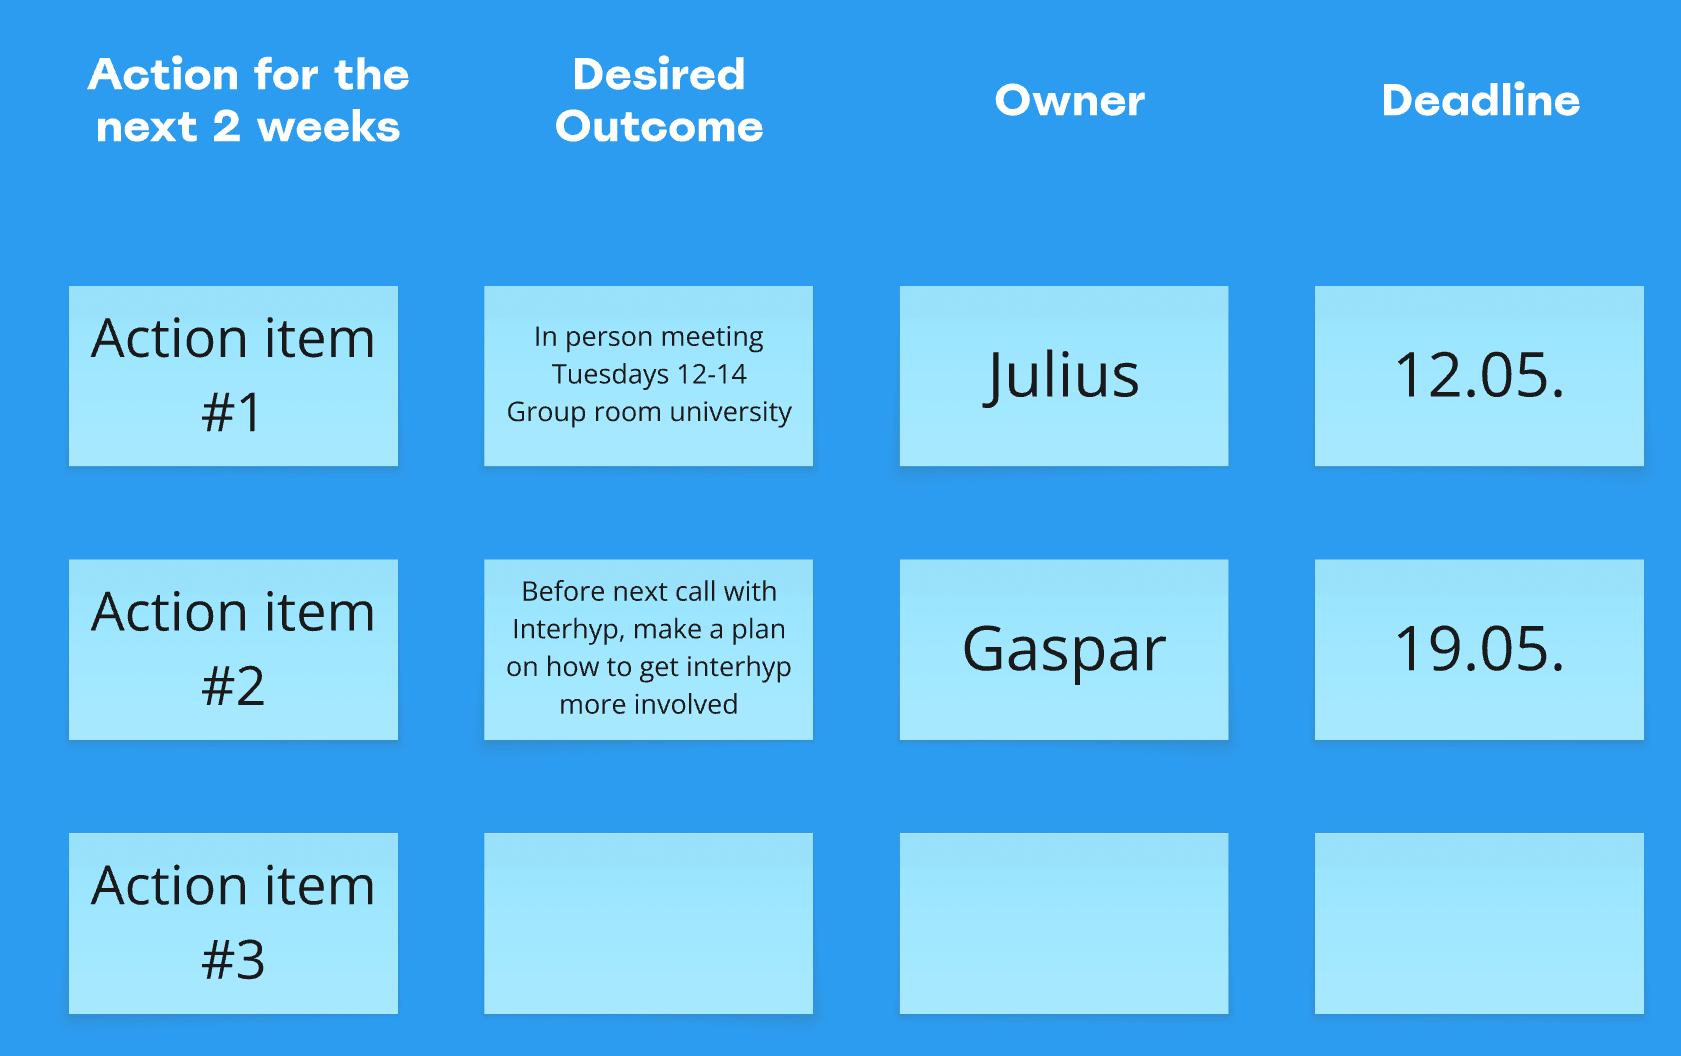
\includegraphics[width=1\linewidth,height=\textheight,keepaspectratio]{assets/sprints/sprint1-retrospective-actions.png}
\captionof{figure}{Sprint 1 retrospective action items showing owners and deadlines.}
\label{fig:sprint1-retrospective-actions}
\end{center}
